\documentclass[12pt, titlepage]{article}

\usepackage{booktabs}
\usepackage{tabularx}
\usepackage{hyperref}
\usepackage{graphicx}
\usepackage{subcaption}
\hypersetup{
    colorlinks,
    citecolor=black,
    filecolor=black,
    linkcolor=red,
    urlcolor=blue
}
\usepackage[round]{natbib}

\title{SE 3XA3: Software Requirements Specification\\Red Discord Bot}

\author{Team \#31, R-DB V2
		\\ Jason Tsui tsuij8
		\\ Student 2 name and macid
		\\ Student 3 name and macid
}

\date{\today}


\begin{document}

\maketitle

\pagenumbering{roman}
\tableofcontents
\listoftables
\listoffigures

\begin{table}[bp]
\caption{\bf Revision History}
\begin{tabularx}{\textwidth}{p{3cm}p{2cm}X}
\toprule {\bf Date} & {\bf Version} & {\bf Notes}\\
\midrule
Oct 4,2018 & 1.0 & Project Drivers, Scope\\
Oct 5,2018 & 1.1 & Added individual use case diagram and function requirements\\
Date 2 & 1.1 & Notes\\
\bottomrule
\end{tabularx}
\end{table}

\newpage

\pagenumbering{arabic}

This document describes the requirements for software project R-DB V2 for McMaster University 3XA3 FALL 2018.\\

The template for the Software
Requirements Specification (SRS) is a subset of the Volere
template~\citep{RobertsonAndRobertson2012}.



\section{Project Drivers}

\subsection{The Purpose of the Project}
Discord is an application which allows people to host and connect with numerous people into a single community over the internet. In these communities, they are able to communicate with each other by talking or typing in text. Oftentimes these communities grow to have over hundreds of persons and the need for community moderation becomes exponentially difficult. The purpose of R-DB V2, is to provide a means of automating commands to moderate the community, enforce rules, and provide community interaction. 

\subsection{The Stakeholders}

\subsubsection{The Client}
	The client of our product is McMaster University who will be the constantly reviewing R-DB V2 and providing guidance to properly document and redeploy the program.

\subsubsection{The Customers}
	The customers of our product are Discord community moderators and owners. The typical owner and moderator would be persons who oversee a large community with numerous members. It is assumed that owners and moderators are looking to automate certain tasks and provide additional functionalities to their community. 


\subsubsection{Other Stakeholders}
Other stakeholders include Discord inc. who will be providing the framework, environment and API to integrate the R-DB V2 program. They are interested in the success of this project as the bot will provide additional user interface and features to the Discord application.

\subsection{Mandated Constraints}
Description: The product shall run on the Discord applcation API and software\\
Rationale: The product is an additional feature intended for the Discord application\\
Fit criterion: Our bot will be available to all users who use the Discord application\\\\

\noindent
Description: The product shall only operate when connected to the internet\\
Rationale: Discord is an online server voIP and thus the product will also be dependant on internet connection\\
Fit criterion: The product shall only operate if an internet connection is present\\

\subsection{Naming Conventions and Terminology}
\begin{itemize}
\item Bot, Autonomous computer controlled program 
\item VoIP, Acronym which refers to Voice over Internet Protocol. Methodology of communication. 
\item Discord, The VoIP platform that is used for the bot.
\item Host, Store a website or data on a server or other computer so that it can be accessed over the internet.
\item Input, User typed in input into Discord community chat.
\item Song request, to request the bot to play a particular song
\item Moderate, Administrative duties to maintain community rules and integrity
\item Kick, to completely remove a user from a community indefinitely
\item ban, to place restrictions on a user in a community indefinitely 
\item softban, to place a ban for a short time
\item stream, to broadcast realtime
\end{itemize}

\section{Functional Requirements}

\subsection{The Scope of the Work and the Product}

\subsubsection{The Context of the Work}
Project is to produce a Discord bot that is able to automate built-in Discord interfaces and provide additional features. Project is expected to be completed by Winter 2018. The exact details for milestones and goals is under the Development Plan and associated Gantt Chart. 

\subsubsection{Work Partitioning}
Group members are expected to equally contribute. Work tasks will be discussed and partitioned on a meeting-by-meeting basis. Work tasks will be generated on a weekly basis based on goals within the most current Gantt Chart and Development Plan.

\subsubsection{Individual Product Use Cases}
\begin{figure}
   \centering
   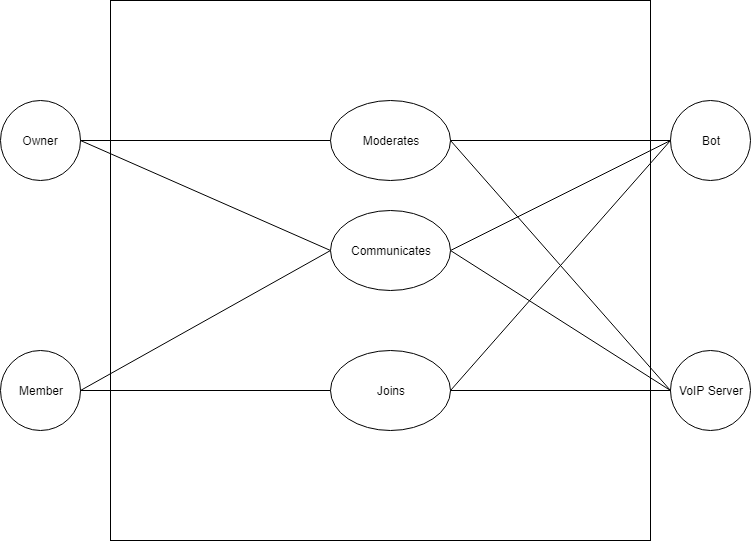
\includegraphics[width=\linewidth]{UseCaseDiagram.png}
   \caption{Use Case Diagram}
  \label{fig:use Case Diagram}
\end{figure}

\subsection{Functional Requirements}
\begin{itemize}
\item The product shall be able to handle music requests and features
\item The product shall be able to host community trivia
\item The product shall be able to kick, ban, and softban users
\item The product shall be able to perform chat cleanup and filtering
\item The product shall be able to produce stream alerts for streaming platforms
\item The product shall be able to perform slot machine functionalities
\item The product shall be able to perform custom commands created by the moderator/owner
\end{itemize}


\section{Non-functional Requirements}

\subsection{Look and Feel Requirements}

\subsection{Usability and Humanity Requirements}

\subsection{Performance Requirements}

\subsection{Operational and Environmental Requirements}

\subsection{Maintainability and Support Requirements}

\subsection{Security Requirements}

\subsection{Cultural Requirements}

\subsection{Legal Requirements}

\subsection{Health and Safety Requirements}

This section is not in the original Volere template, but health and safety are
issues that should be considered for every engineering project.

\section{Project Issues}

\subsection{Open Issues}

\subsection{Off-the-Shelf Solutions}

\subsection{New Problems}

\subsection{Tasks}

\subsection{Migration to the New Product}

\subsection{Risks}

\subsection{Costs}

\subsection{User Documentation and Training}

\subsection{Waiting Room}

\subsection{Ideas for Solutions}

\bibliographystyle{plainnat}

\bibliography{SRS}

\newpage

\section{Appendix}

This section has been added to the Volere template.  This is where you can place
additional information.

\subsection{Symbolic Parameters}

The definition of the requirements will likely call for SYMBOLIC\_CONSTANTS.
Their values are defined in this section for easy maintenance.


\end{document}